%&latex
\documentclass[12pt]{article}
\usepackage{amsthm,amsmath}
\usepackage{graphicx,psfrag,epsf}
\usepackage{enumerate}
\usepackage{natbib}
\usepackage{url} % not crucial - just used below for the URL
\usepackage{amsthm,amsmath}
\usepackage[utf8]{inputenc}

%\pdfminorversion=4
% NOTE: To produce blinded version, replace "0" with "1" below.
\newcommand{\blind}{0}

% DON'T change margins - should be 1 inch all around.
\addtolength{\oddsidemargin}{-.5in}%
\addtolength{\evensidemargin}{-.5in}%
\addtolength{\textwidth}{1in}%
\addtolength{\textheight}{1.3in}%
\addtolength{\topmargin}{-.8in}%


\begin{document}

%\bibliographystyle{natbib}
%\bibliographystyle{bmc-mathphys}
\bibliographystyle{agsm}

\def\spacingset#1{\renewcommand{\baselinestretch}%
{#1}\small\normalsize} \spacingset{1}


%%%%%%%%%%%%%%%%%%%%%%%%%%%%%%%%%%%%%%%%%%%%%%%%%%%%%%%%%%%%%%%%%%%%%%%%%%%%%%

\if0\blind
{
  \title{\bf Approachable case studies support learning and reproducibility in data science: An example from evolutionary biology}
  \author{Luna L. Sanchez Reyes\thanks{
    The authors gratefully acknowledge ``Sustaining the Open Tree of Life``, NSF ABI No. 1759838, and ABI No. 1759846.}\hspace{.2cm}\\
    School of Natural Sciences, University of California, Merced\\
    and \\
    Emily Jane McTavish \\
    School of Natural Sciences, University of California, Merced}
  \maketitle
} \fi

\if1\blind
{
  \bigskip
  \bigskip
  \bigskip
  \begin{center}
    {\LARGE\bf Approachable case studies support learning and reproducibility in data science: An example from evolutionary biology}
\end{center}
  \medskip
} \fi

\bigskip
\begin{abstract}
Research reproducibility is essential for scientific development. Yet, rates of reproducibility
are low, especially in the natural sciences. As increasingly more research is relying on
computing tools and software, efforts for improving
reproducibility rates have focused on making available research workflows
as computer code, as well as raw and processed data in computer readable form.
However, research products that are digitally available are not necessarily
friendly for learners and interested parties with little to no %%% different levels of
experience in the field. This renders research products unapproachable, which
counteracts availability, and hinders reproducibility short and long term.
To improve long term adoption of reproducible workflows in research, they
need to be made approachable for learners, the researchers of the future.

Using an example within evolutionary biology, we identify aspects of research workflows
that make them unapproachable to the general audience:
use of specialized computing language and programming techniques;
high cognitive load;
unspecified, unclear or lengthy goals;
content-focused descriptions instead of user-focused;
inflexible learning environment;
unapproachable (cold or intimidating) language; and
little to no diversity of representation of information.
Then, we propose a set of principles to improve the unapproachable aspects of
research workflows, and illustrate their application in a case study from
evolutionary biology that we used as teaching material.
Finally, we elaborate on the general application of these principles for
documenting research workflows and products, to provide present learners
and future researchers with tools for successful scientific reproducibility.
%> ** add a sentence on implications for teaching reproducibility


%% Projects that address availability of code and data in the natural sciences
%% have focused on producing documentation that describes the nature and usage of the
%% resources.
%% However, it is often written using highly specialized language that is largely
%% inaccessible for the average target user. Additionally, baseline
%% computational knowledge and skills required to access scientific results are often
%% not found among potential users, and keep on increasing.

\end{abstract}

\noindent%
{\it Keywords:}  open science, R, phylogenetics, Open Tree of Life
\vfill

\newpage
\spacingset{1.45} % DON'T change the spacing!
\section*{Introduction}
\label{sec:intro}

Research reproducibility --the extent to which consistent results are obtained when
a scientific experiment or research workflow is repeated \citep{repdef2021}--
is a key aspect of the advancement
of science, as it constitutes a minimum standard that allows understanding research products,
i.e., methods, data, analysis, results, etc. \citep{piwowar2013value},
to determine their reliability and generality, and eventually build up scientific
knowledge and applications based on those products
\citep{king1995replication, peng2011reproducible, powers2019open}.
In the natural sciences, rates of reproducibility are low \citep{ioannidis2005most, prinz2011believe},
which has elicited concerns about a crisis in the field \citep{baker2016reproducibility}.

In response, the scientific community has been developing new principles and standards to incentivize
cultural changes that support a long term improvement of reproducibility rates in the natural sciences
\citep{peng2015reproducibility, wilkinson2016fair, miyakawa2020no}.
A standard for reproducibility that has received much attention is availability, which
we define as a property denoting that a research product can be reached (acquired, copied, analyzed,
processed and/or reused) at no financial, legal or technical cost \citep{arnold2019turing},
and without geographic, demographic, social or temporal barriers for the population \citep{fecher2014open}.

In this paper, we argue that research products that are digitally available are
often unapproachable in practice (Box 1), because they are not
friendly for learners and interested parties with different levels of
experience in the field. Research products that are unapproachable
counteract availability, and hinder reproducibility short and long term.
To support long term adoption of reproducible practices in the natural sciences, research
workflows need to be made approachable for learners, the researchers of the future.

To elaborate on our thesis, we designed a case study within the research field of
phylogenetics, a discipline within evolutionary biology.
We use our case study to identify barriers that have made research workflows
largely unapproachable to a general audience in the natural sciences.
Then, we propose some principles for researchers to address these barriers, and
create research workflows that are reproducible by a larger audience.
% ** describe/introduce reproducibility curriculum here
The principles proposed here can be generalized and integrated into the undergraduate
and graduate school STEM curriculum, either for courses specialized in reproducibility
or within other subject areas, as a necessary component of successful and impactful science.

%% \bigskip
%% \bigskip
%%
%% \noindent\fbox{%
%%     \parbox{\textwidth}{%
%%     \textbf{Box 1. The role of approachable research workflows in teacing reproducibility.}
%%       % Availability is defined as the fact or possibility that something can be bought,
%%       % used, or reached by someone \citep{availability2022cambridge}.
%%       % Accessibility is defined as "the fact of being able to be reached or obtained easily"
%%       % \citep{accessibility2022cambridge}
%%       % Yet, in practice, availability does not imply accessibility.
%%       Availability and accessibility are conceptually accepted as synonyms for ``the fact
%%       of being able to be reached" \citep{available-accessible2022cambridge}.
%%       However, accessibility's definition goes further and describes it as the
%%       ``fact of being able to be reached \textbf{easily}" \citep{accessibility2022cambridge}.
%%       A secondary definition of accessibility elaborates more on this: ``the quality
%%       of being \textbf{easy to understand}''.
%%
%%       What we realize from these definitions is that, in practice, something might
%%       be available but not necessarily accessible,
%%       hindering the realization of availability.
%%       To illustrate the practical difference between availability and accessibility we
%%       will use an allegory that goes like this:
%%
%%       ** Change marshmallow story to cake
%%
%%       ** Explain different types of barriers to accessibility within the example, then within science
%%
%%       ** Explain why we focus on psychological/social/pedagogical barriers
%%
%%       ** Gauging accessibility of a resource is tricky because it depends on an
%%       individual experience of what is in effect \textbf{easy} for someone.
%%       \textbf{Easy} is a subjective quality that fully depends on individual perceptions
%%       resulting from individual contexts.
%%       As a society we are moving towards validating and welcoming all human experiences.
%%       To improve accessibility levels in the natural sciences, it
%%       is important to account for the factors that are creating different experiences
%%       of what is \textbf{easy}.
%%
%%       ** Now, explain different types of barriers to accessibility in science
%%       (Jessica: Maybe say that lack of accessibility can be due to a number of
%%       factors (physical, resources, economic), but one critical factor is the use
%%       of impenetrable expert language.)
%%     }%
%% }
%% \bigskip

\bigskip
\bigskip

\begin{figure}
\begin{center}
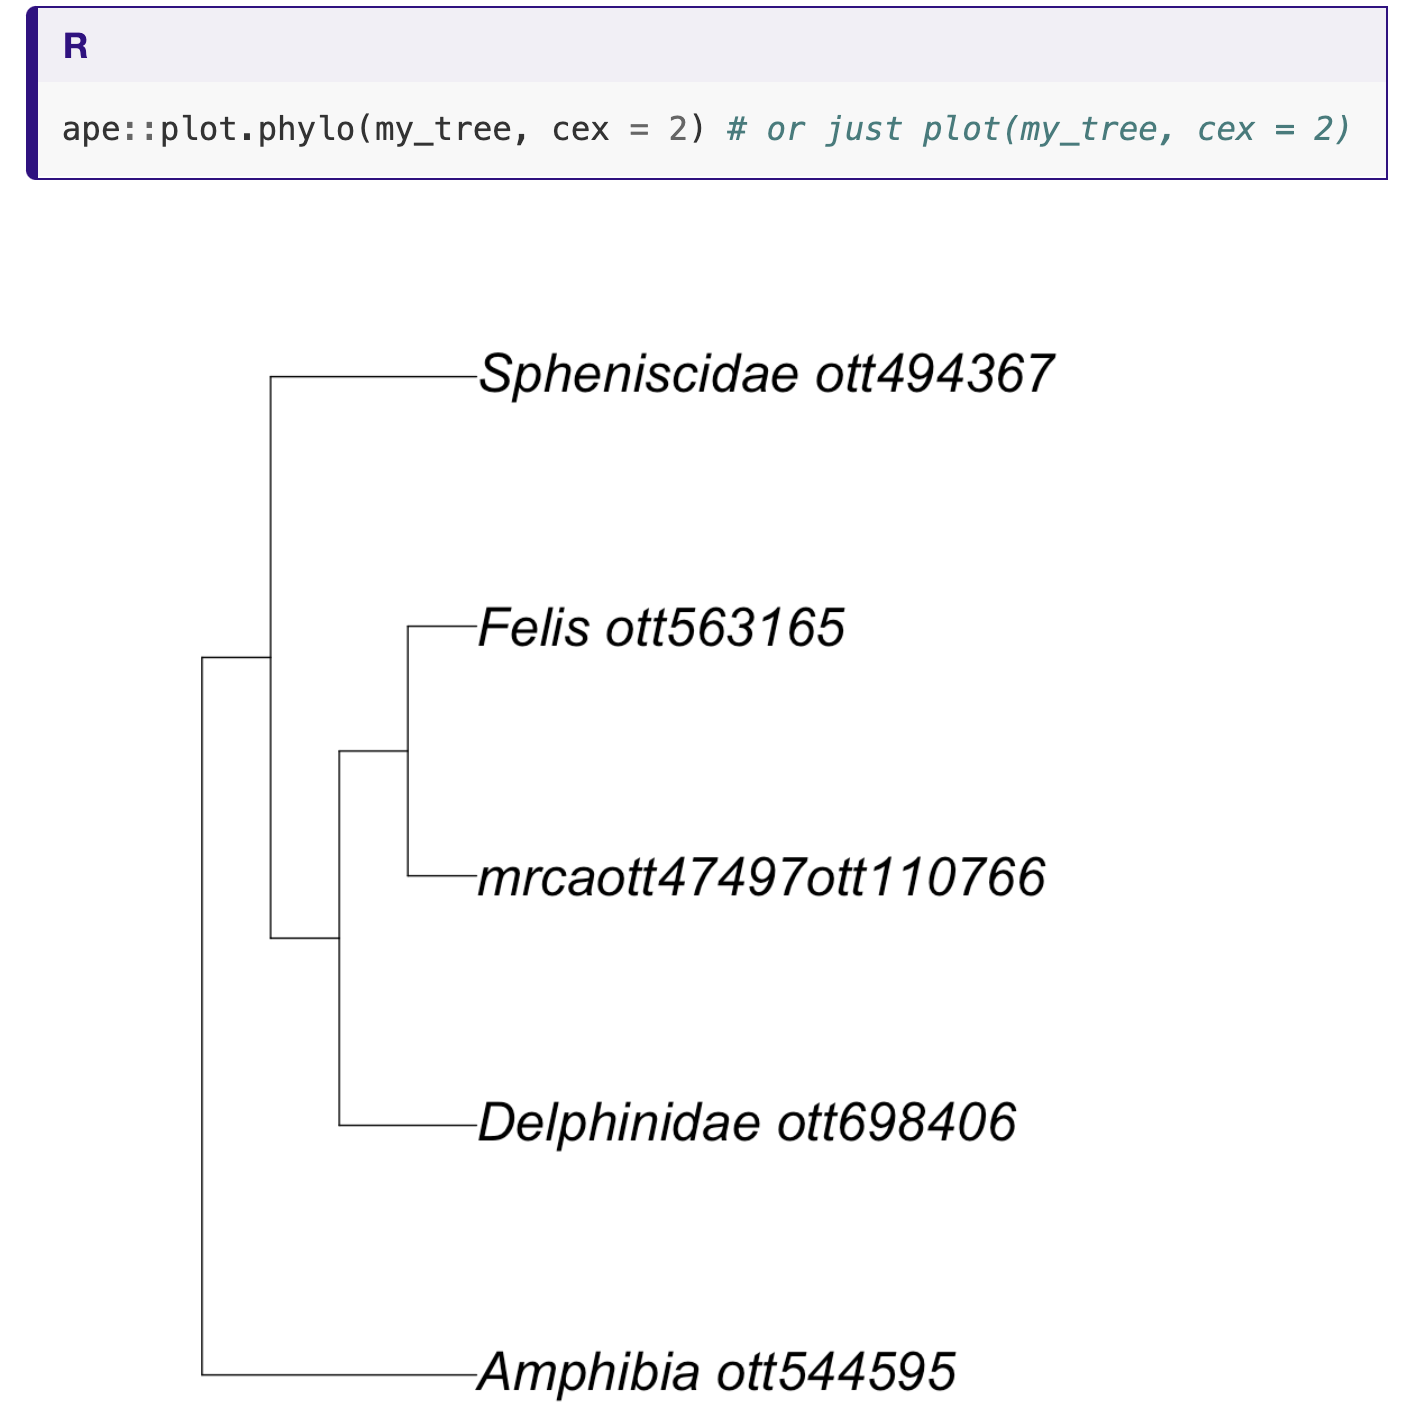
\includegraphics[width=3in]{fig-tree.png}
\end{center}
\caption{A phylogenetic tree from our tutorial. It was extracted using OpenTree of Life resources \citep{opentreeoflife2019synth} wrapped in the \texttt{rotl} R package \citep{michonneau2016rotl}. \label{fig:tree}}
\end{figure}

\section*{A case study from phylogenetics}
\label{sec:case}

Phylogenetics is a key discipline within evolutionary biology \citep{dobzhansky1973nothing}.
It focuses on investigating the history of shared ancestry of living and extinct
organisms using biological data,
and represents this evolutionary history with a diagram known as a phylogeny
or phylogenetic tree (because it grows through time and appears to have branches;
Figure \ref{fig:tree}).
Phylogenies provide the basis to study and understand all biological processes
in an evolutionary context \citep{dobzhansky1973nothing}
Hence, it appears that improving reproducibility rates in phylogenetics has the
potential to positively impact research across the natural sciences.

To explore barriers to approachability in phylogenetics, we develop a case study
that touches on three common problems within the field: standardizing
organism names in phylogenies, obtaining current phylogenetic knowledge for a group of organisms,
and summarizing this phylogenetic knowledge in a meaningful way.
To address these problems, we propose a research workflow that relies on resources from the Open
Tree of Life (OpenTree), an open source project that provides
digital availability of phylogenetic results from published, peer-reviewed research, which
is considered as vetted and state-of-the-art knowledge in the field.
OpenTree phylogenies are stored in a public database, the Phylesystem \citep{mctavish2015phylesystem},
and are downloadable as various computer-readable file types, which is key for reusability
and reproducible workflows \citep{wilson2017good}.
OpenTree also provides access to a single naming standard for organisms (taxonomic standard)
that is applied to the stored phylogenies \citep{rees2017automated}, which are
then used to summarize a single phylogenetic tree encompassing all life \citep{opentreeoflife2019synth}.

All of OpenTree resources
%% (the stored phylogenies, the taxonomic standard, the synthetic tree, and all
%% tools developed to process and summarize stored phylogenies),
are free of cost to any user, and are available for download and use through its Graphical User
Interface (GUI; aka, a website or application that allows users to access computer functionalities, in this case OpenTree resources, with mouse or keyboard clicks).
However, reducing as many manual steps as possible in research workflows is key
for reproducibility, as manual data manipulation scales poorly and is prone to
error \citep{bakken2019journey}.
OpenTree's resources are also programmatically available through its Application
Programming Interface services (APIs; aka, computer code that implements computer functionalities,
in this case OpenTree resources, that can be used by programmers
to build more functionalities),
which provide scalability and reproducibility \citep{opentreeAPIv3}.
However, this comes at a high cost for the user, which requires considerable more
computer programming experience and literacy to be able to successfully use APIs.
%% In recent years, OpenTree API services have been wrapped into software packages for R and Python
%% \citep{michonneau2016rotl, mctavish2021opentree}, open source, free of cost
%% programming languages that represent two of the most widely used programming languages
%% in the sciences \citep{baker2017scientific}. These packages should contribute to making
%% OpenTree resources more accessible to a wider user audience.
The \texttt{rotl} R package \citep{michonneau2016rotl} and the \texttt{opentree} Python module
\citep{mctavish2021opentree} have been developed as wrappers for OpenTree's API services.
R and Python are open source and free of cost programming languages that represent
two of the most widely used programming languages in the sciences today \citep{eglen2009quick, baker2017scientific}.
As such, \texttt{rotl} and \texttt{opentree} software packages should contribute
to making OpenTree resources more accessible to a wider programming user audience.

However, while learners in the natural sciences have been engaging independently
with R and Python programming languages, computer programming is not traditionally
a core skill formally taught to biologists and naturalists
\citep{sayres2018bioinformatics, wright2019the, williams2019barriers}.
As computers continue to play a larger role in most scientific disciplines \citep{piccolo2016tools},
higher baseline computational skills are required across all natural sciences not only
to develop an original research workflow, but to be able to follow and reproduce
research workflows from other researchers.

Thus, efforts to increase reproducibility rates long term in the natural sciences
would benefit from addressing specific barriers for learners in the field, to
support them in acquiring the skills needed to reproduce research workflows
that rely heavily on computer code \citep{peng2011reproducible, sandve2013ten, powers2019open}.

In the next section, we describe the barriers to approachable research workflows that we identified
on our case study. We address these barriers in a set of teaching materials that are
available at
https://mctavishlab.github.io/R\_OpenTree\_tutorials/.


\section*{Identifying barriers to approachable research workflows}
\label{sec:identifying}

% Cite carpentries and Mosi

The main goal of our research workflow is to obtain a single phylogeny summarizing
data from a set of published phylogenies for the canids (the family of dogs, coyotes, wolves, etc.),
our organism of study.
Our analysis can be completely accomplished using functions
from the R package \texttt{rotl} or the Python module \texttt{opentree}. If
a researcher were to use this workflow in a publication, they would typically
describe it in the methodology section as ``The canid summary phylogeny was obtained using
functions from X package, details are available as supplementary files".
This is usual practice, mainly because journals do not have space to publish
all code used in an analysis in the methods section. Yet, supplementary files have
the misfortune to not be peer-reviewed as thoroughly (or at all) as the main manuscript
\citep{CITATION}.
They are also prone to the dreaded promise ``available upon request", which has
very low rates of fulfillment \citep{CITATION}.
Without the primary code that was used to perform an analysis it is impossible
to reproduce said analysis. When the code is available, other issues can
complicate reproduction of the analysis to the point of completely obstructing
reproducibility.
For example, what software do I need to open the code files? Can I run the code within the same
software, or do I need a different one?
Do I need additional software that the analysis depends on? What does the code even mean?

These questions are usually addressed in the software documentation.
As opposed to code, documentation is written in natural language (i.e.,
any known human language, e.g., English, Spanish, Chinese), and is considered
a key element for successful adoption of software
by the target users \citep{karimzadeh2018top}. This might explain
why documentation for software addressed to academic users is also
usually written using highly specialized computational
language or jargon (i.e., computationally specific concepts,
words, and phrases) as well as formal scientific and academic language.
\textit{Barrier 1.--} While scientific jargon might have an important role for formal acceptance
of software by the scientific and academic community, it can be perceived as
cold and/or intimidating language, that often slows down or even
obstructs examination, application, and adoption of code by a wider audience \citep{ball2017its},
and discourages learners by creating a hostile environment that does not foster learning \citep{CITATION}.

Good software documentation for code has to be thorough \citep{karimzadeh2018top}.
It should describe general usage of individual functions, as well as
the argument and variables said function can take, and it should be accompanied with
usage examples on how to apply each function \citep{karimzadeh2018top}.
Individual documentation for each function is usually presented
in alphabetic order, and does not have a specific goal, besides being as thorough as possible.
In this context, identifying connections across functions that are meant to work on the same
analysis workflow is difficult. Moreover, most software has many functions, so documentation
is usually very lengthy. \textit{Barrier 2.--}  All of this increases the cognitive
load for the target users and learners, which discourages learners \citep{CITATION}.

Another important aspect of software documentation is that examples are usually
worked and showcase the ideal or minimal case in which a function should work well.
\textit{Barrier 3.--} Focusing importance on the content of the software instead
of considering the user experience, ignoring what can go wrong and avoiding clear
advice on how to troubleshoot.

Software documentation is usually explained with words, very rarely using diagrams or
other allegories.
\textit{Barrier 4.--} Little to no diversity of representation of information

Documentation should always be available for the users and learners
\textit{Barrier 5.--} Inflexible learning environment, is this one really an issue???




% Some principles of an inclusive syllabus:

% - unspecified, unclear or lengthy goals; high cognitive load; (literate programming)

% - content-focused descriptions/examples instead of user-focused; (demonstrate errors)

% - inflexible learning environment; (make it stable so users can learn whenever is best for them)

% - unapproachable (cold or intimidating) language, use of highly specialized computing jargon, skill level; (use friendly and informal but respectful language)

% - and little to no diversity of representation of information (say the same thing with different images, metaphors, stories)

In sum, best practices for good primary documentation are not enough to ensure
reproducibility of research workflows that rely heavily on code.

\section*{Best practices for approachable research workflows}
\label{sec:addressing}

\subsubsection*{a. Reduce cognitive load and provide specific and clear goals
with literate programming}

Pedagogical research shows that active learning practices are one the most effective
ways to take on abstract subjects \citep{freeman2014active}.
Programming computer languages are quite abstract and cognitive load can be greatly
reduced for learners by applying an active learning strategy such as linking its usage to
a ``real world'' or ``human'' application \citep{felder2009active}.

A story-like narrative that links code usage in an integrative example, invites learners
to try the code, which can lead them to remember what they are doing and
why they are doing it.
This ``literate programming'' paradigm \citep{knuth1984literate, fritzson2002mathmodelica}
makes code more approachable, as it integrates narratives with computer code in
the same document, supporting learners in actively following
the code usage, supporting memory and understanding \citep{piccolo2016tools}.

We propose that documents developed with ``literate programming'' can be made more
accessible by choosing narratives that are relatable to a more general audience.
An easy way to do this in biology is choosing a charismatic taxon as model organism.
For a research group this can be the group they are studying. For the general audience,
a highly charismatic group such as dinosaurs will do the trick.


We examined available primary documentation for the package \texttt{rotl},
and designed a narrative that required the usage of as many functions as possible.
We demonstrate code applications that are commonly requested by OpenTree users,
but that are not demonstrated in the primary documentation of the R package.
By framing the function workflow using highly requested uses, the documentation acquires a
narrative arc that is easier to follow and remember by users. This can also facilitate
the application of code to other use cases in biology of interest for the users.

%% Maybe Figure!! For the tutorial demonstrated here, we used the commonly requested
%% use case of obtaining
%% a phylogenetic tree for all lineages within a specific taxonomic rank.

\subsubsection*{b. Provide examples that are user-focused by demonstrating errors and warnings}

% approachable practice: user focused examples (instead of content focus)
% demonstrate errors and warnings thoroughly

A practice that has become more and more widespread in programming-language pedagogical practices
is the use of typos and mistakes to normalize them for learners, and show them how
to solve them when they are outside the classroom \citep{shannon2015live}.
Yet, this is rarely done on written pedagogical materials.
Primary documentation focuses on demonstrating usage function with examples that
work seamlessly, without errors. We argue that the opposite is needed to support
adoption of reproducible workflows and support long term independence in learners
\citep{gaspar2007restoring}.
We demonstrate examples that do not work
as expected and exemplify ways to address them (Figure \ref{fig:error}).

We identify inputs that would give
a wide range of warnings and errors, focusing on demonstrating these cases. This
helps users to not be afraid of errors and warnings, but instead to use them to
their advantage.
We also identify effects of warnings and errors downstream of the workflow.

We identify ways to evaluate inputs to know if they will produce an error, and design
alternatives on what to do when faced with an error or warning, and demonstrate
these alternatives.
One of the most essential skills in programming is interpreting and moving forward
from errors.
Many finely honed tutorials do not trigger errors, which precludes helping students
to develop the tools to understand and address errors when they do encounter them,
as they inevitably will.
In our tutorial, we focus on explaining the meaning and downstream of warnings and errors, and
 showcase ways to detect them before they are triggered (i.e., before using an input
  that would elicit a warning or error). This has two pedagogical benefits:
1) it provides users/students with the means to troubleshoot their own warnings and errors, and
2) it allows users/students to understand with more depth what the function is doing.

% We designed ways to access the different elements of the outputs.

\begin{figure}
\begin{center}
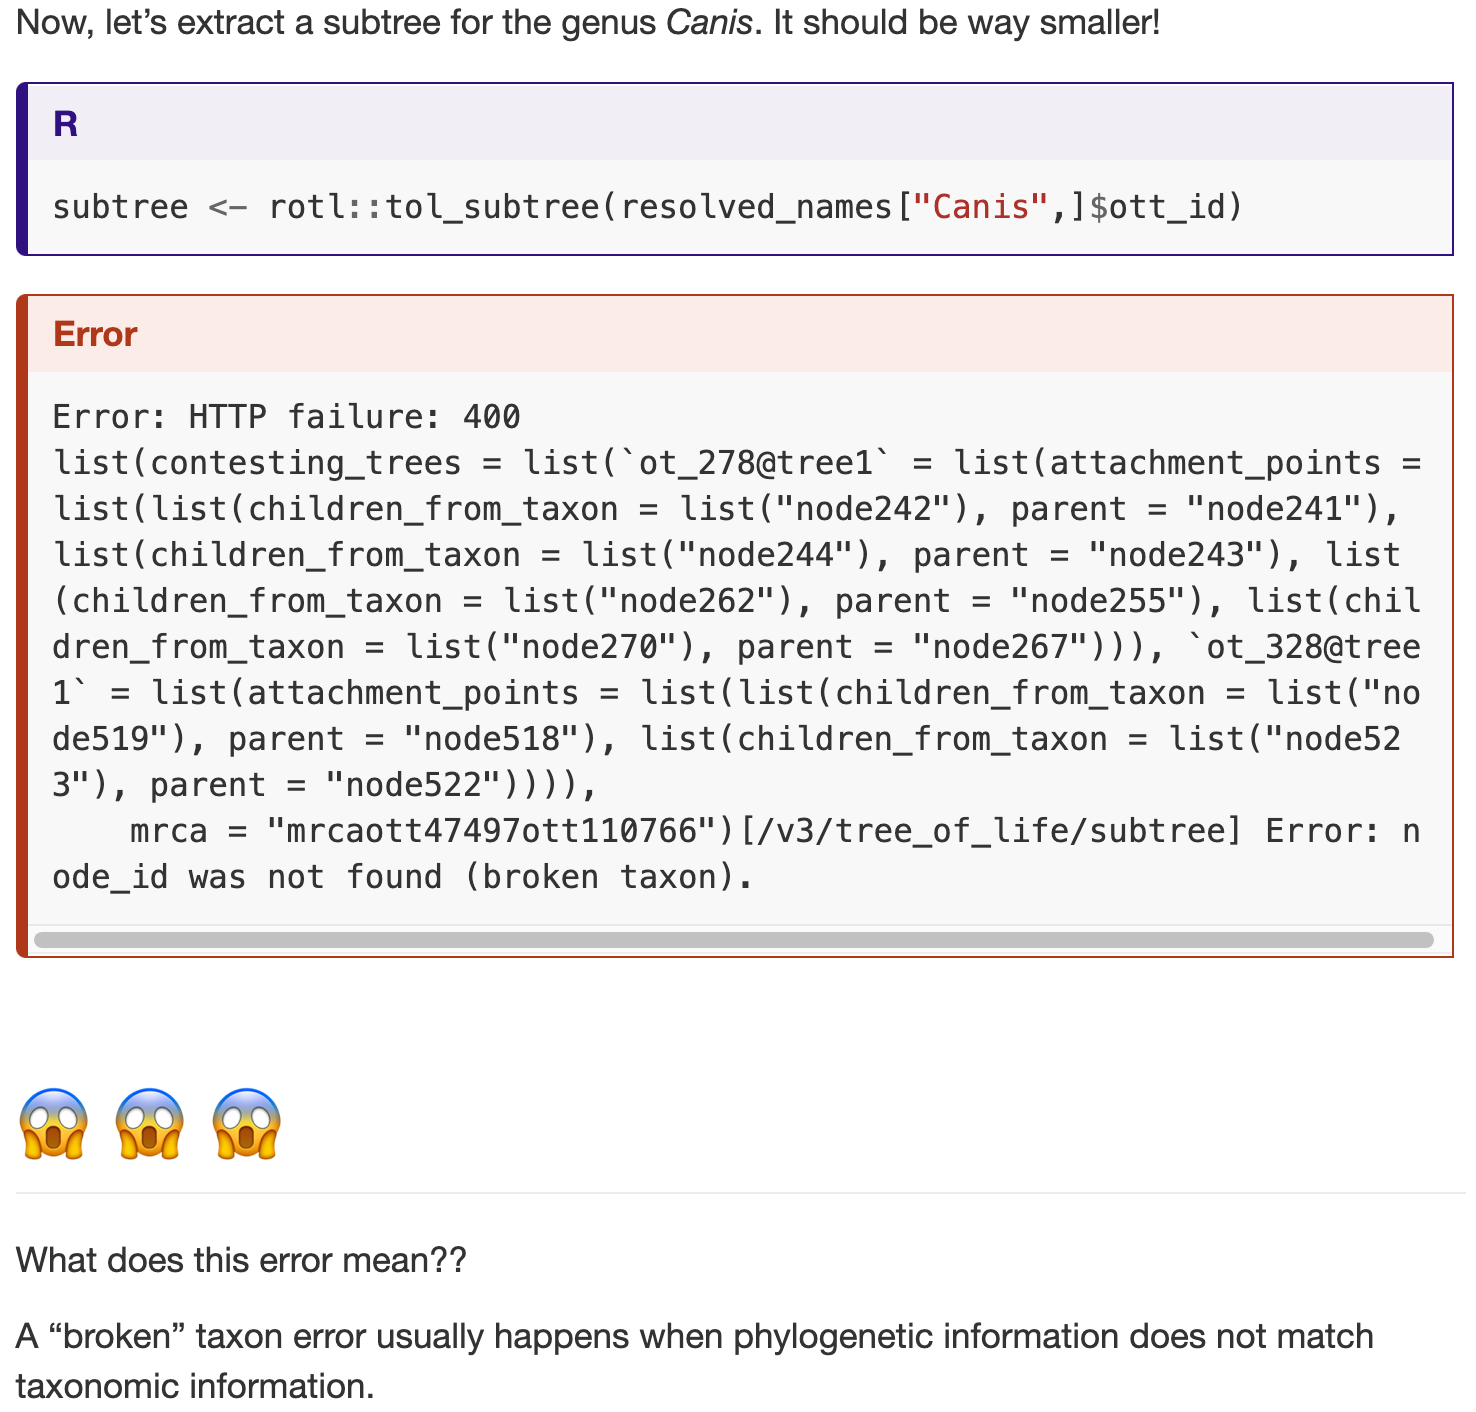
\includegraphics[width=3in]{fig-error.png}
\end{center}
\caption{Snapshot of a section of the tutorial website, where we demonstrate a common error. \label{fig:error}}
\end{figure}

\subsubsection*{c. Use friendly, relatable and respectful language}

% avoid specialized, intimidating and cold language

Besides avoiding formal language, and incorporating elements of pop culture, such as picture
character icons known as ``emojis``, to make the language more familiar to a
broader target audience (see Figure \ref{fig:error}), we made an effort to specifically
complement the primary documentation by identifying
computational concepts that were assumed or were not explained in depth.
We vetted the tutorials through feedback from workshop participants as well as
individual users to identify such specialized concepts.



\subsubsection*{d. Make it accessible geographically and through time}

% - inflexible learning environment; (make it stable so users can learn whenever is best for them)

We published the tutorials on a public, free license, free of cost, and free for
use and reuse repository and persistent website \citep{RopentreeTutorials}.
The tutorial is available for the users to go back to any time they need it,
and to be passed on to other users (Figure \ref{fig:schedule}).

\begin{figure}
\begin{center}
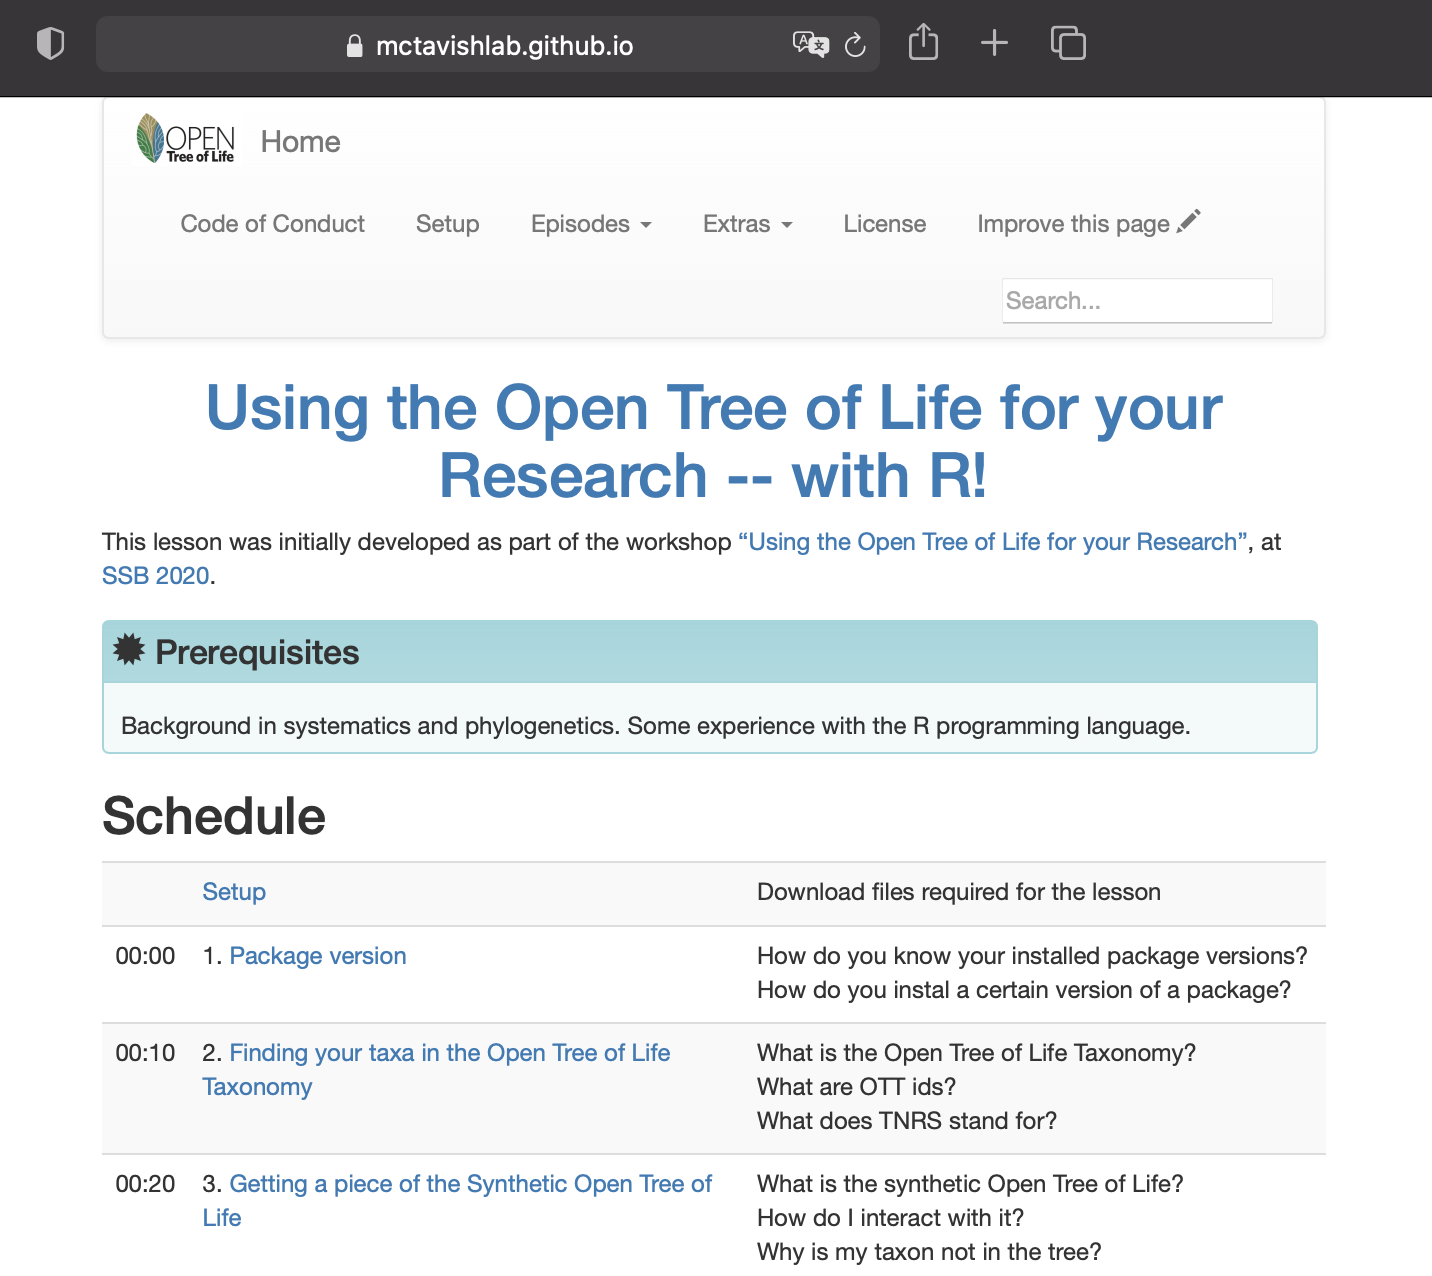
\includegraphics[width=3in]{fig-schedule.png}
\end{center}
\caption{Snapshot of the home to our tutorial website, showing part of the schedule. \label{fig:schedule}}
\end{figure}

We created a main version of the tutorial that is stable. Any updates to the tutorial are
published as new versions, or tutorials for new workshops \citep{wilson2006swc, SWCwebsite}
 Versions presented at workshops are a copy from the original repository.
They represent a temporally stable snapshot of functions and workflows presented
during a workshop.

%%% \subsubsection*{5. The (now) classics of computational reproducibility}
%%%
%%% Provide all information on package version and system capabilities.
%%%
%%% > [name=Emily Jane McTavish]link to where/and how you did that

\section*{Conclusion}
\label{sec:conclusion}

Response form the community has been invaluable in gauging success of our teaching
materials.
Senior researchers often comment on the usefulness
of the tutorials for their research, as well as how they have supported students in using the
R packages with less help from them as PIs.

Making accessible reproducible workflows has several advantages:

* save explanation/training time when analyses are run again by students and collaborators;
* save research time for yourself when analyses are run again with more data, a* different dataset, a different organism or biological model;
* scientific efforts can build off of each other.


Ultimately, the long term improvement of reproducibility rates in science will depend
on our ability to intentionally integrate the subject of reproducibility into the
undergraduate curriculum, so college learners and future researchers have the
basis to develop the fundamental skills needed to successfully create reproducible
scientific workflows and materials.

Some universities have been incorporating the subject in their classes (see
\cite{uwlibraries2022, nigms2022}).
The focus of these resources has been for students to develop skills to document their work.
The principles identified and outlined here can be used to set learning goals and
outcomes on new reproducibility syllabi.

The principles to create tutorials described here facilitate adoption of software
 and analysis workflows among researchers at different academic levels, from undergrads
  to established researchers.
It will also help close the gap between students that had access to computational
resources (and computational training) from an early age and students that did not.
Late access to computational resources and training can occur due to lack of
economic resources, often occurring in households from underrepresented communities
and minorities \citep{google2016diversity, warner2021quantifying}.
It can also be due to gender-biased parental and community pressures,
in which male individuals are more often encouraged to perform activities related to computers,
while female individuals are discouraged \citep{warner2021quantifying}.
% How to balance software acceptance VS. adoption?
These principles can be used to improve not only reproducibility practices,
 but also software adoption in the natural sciences.
%% Discuss: why address accessibility and not other aspects of reproducibility?


\bigskip
\begin{center}
{\large\bf SUPPLEMENTARY MATERIAL}
\end{center}

\begin{description}

\item[Title:] Website and GitHub repository containing the complete teaching materials developed and demonstrated here.

\item[GitHub repository link:] \url{https://github.com/McTavishLab/R_OpenTree_tutorials}

\item[Website link:] \url{https://mctavishlab.github.io/R_OpenTree_tutorials}

\end{description}

\bibliography{Manuscript-bibliography}

\end{document}
